\documentclass[a4paper, 11pt]{article}
\usepackage[utf8]{inputenc}
\usepackage[T1]{fontenc}
\usepackage[french]{babel}
\usepackage{hyperref}
\usepackage{graphicx,float}
\usepackage{fixltx2e}


\hypersetup{colorlinks,linkcolor=black,urlcolor=blue}

\begin{document}

\title{Design Pattern : Pacman}
\author{Théo \textsc{DÉZÉ}  \& Charles \textsc {MALLET}}
\date{20 Décembre 2018} 


\maketitle

\vspace{2cm}
\begin{figure}[ht]

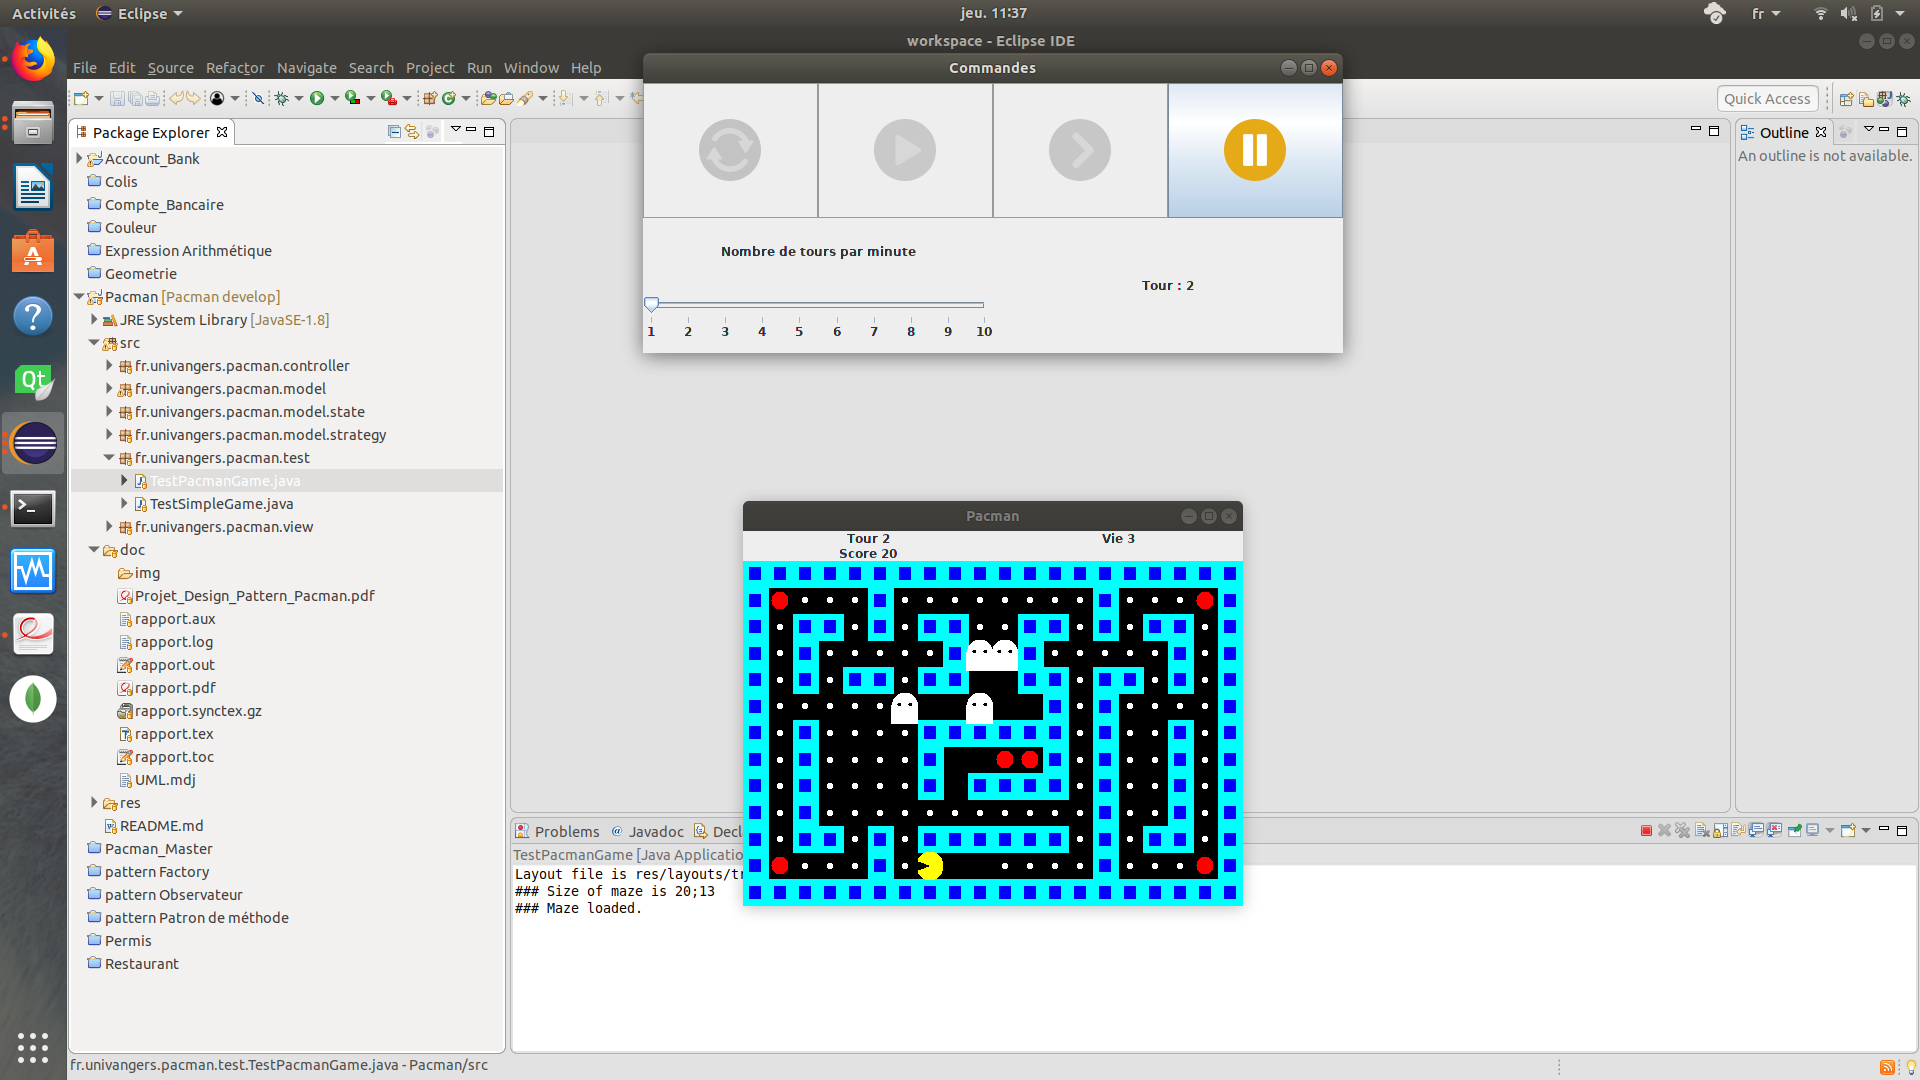
\includegraphics[scale=0.7,trim=26.2cm 5cm 23.9cm 17.7cm, clip=true]{img/Pacman.png}

\end{figure}


\newpage

\tableofcontents

\pagebreak

\part*{Introduction}

Au cours des Travaux Pratiques de Design Pattern, nous avions pour projet de recréer le jeu Pacman. Selon les règles de base, le Pacman doit chercher la nourriture dispersée aux quatre 
coins de la map tout en évitant les fantômes qui veulent l'attraper. Pour s'aider, les pacmans peuvent utiliser des capsules les rendant invulnérables et leur octroient 
la possibilité de tuer les fantômes pour un temps limiter.

Codé en JAVA à l'aide de l'IDE Eclipse, nous devions implémenter les différentes fonctionnalités du célèbre jeu avec tous les agents d'origine. Nous devions également
proposé une intelligence Artificielle pour les fantômes afin de rendre le jeu totalement fonctionnel. 

Dans ce rapport, nous allons vous présenter les diverses Patterns utilisés. Nous commencerons tout d'abord par vous parler du PacmanGame et de son Pattern MVC. Nous continuerons
avec l'Intelligence Artificielle que nous avons implémenté à l'aide du Pattern Strategy. Ensuite, nous continuerons avec les derniers Patterns exploités pour que notre 
Pacman fonctionne. Enfin, nous concluerons par vous présenter l'état final de notre projet.


\part{PacmanGame et Pattern MVC}
\begin{itemize}
  \item PacmanGame :  \\ 
  
Comme dit précédemment dans l'Introduction, nous avons implémenté les comportements de base du Jeu Pacman. Au sein de la classe PacmanGame, nous avons appelé
les fonctions essentielles à son bon déroulement et créer les différents items utiles au jeu. \\
 
  \item Pattern MVC : \\
  
Le Design Pattern Pattern MVC signifie Modèle-Vue-Controller. Dans le cadre de notre projet, nous avons donc exploité ce concept afin d'améliorer
notre architecture. Dans la Vue, nous avons défini les différentes interfaces grahiques de notre application : la vue du jeu, la vue des commande,
ainsi qu'une interface vue qui permet de mettre à jour le rendu du jeu en fonction des commandes appelées. D'un autre côté, nous avons appelé la
classe PanelPacmanGame que notre professeur Monsieur Goudet nous a donnés pour dessiner le jeu. Dans le Controller, nous avons implémenté les 
fonctionnalités servant à contrôler le jeu, c'est-à-dire les mouvements des agents contrôler par les joueurs ainsi que les widgets de l'interface
graphique permettant, par exemple, de mettre en pause le jeu ou d'augmenter et réduire la vitesse du jeu. Enfin, concernant le Modèle, nous y avons
défini tout ce qui correspondait au fonctionnement même de l'application tels que les classes Agents, FactoryAgent, Game ainsi que les États et Stratégies 
dont nous parlerons plus en détail par la suite. 

\end{itemize}

\part{Intelligence Artificielle et Pattern Strategy}

\begin{itemize}
  \item Algorithme A* : \\
  
L'Algorithme A* est un algorithme de recherche très puissant. Il permet de calculer efficacement le chemin le plus court pour se rendre d'un point I à un Objectif F.
À l'aide d'heuristique, il parcourt un graphe en cherchant le coup de déplacement le plus minimal. Dans le cadre de notre Pacman, il est utilisé
pour les fantômes lorsqu'ils partent à la poursuite du Pacman ainsi que pour échapper à ce dernier lorsqu'il devient invulnérable. Par ailleurs,
Pacman utilise aussi cet algorithme lorsque l'utilisateur demande à ce que l'agent joue automatiquement, au lancement de la partie. \\

  \item Pattern Strategy : \\
  
Le Pattern Strategy nous a été très utile. En effet, il nous a permis de définir les différentes intelligences artificielles des agents fantômes 
du jeu. Ces derniers se servent d'une stratégie d'attaque AstarStrategy lorsqu'ils repèrent le Pacman ainsi qu'une stratégie défini dans la classe 
AstarEscapeStrategy lorsque leur vie est mise en danger par l'absorption d'une capsule.

\end{itemize}

\part{Autres Patterns utilisés}

\begin{itemize}
  \item Pattern Factory : \\
  
Ce Design Pattern nous a été utile dans le cadre de la création des Agents. Grâce à celui-ci nous avons pu facilement créer différent agents avec des
méthodes similaires permettant toutes de créer des fantômes ou des pacmans aux caractéristiques souhaitées. Il a été implémenté grâce à la classe 
FactoryAgent où nous avons défini ces méthodes et appelés lors du lancement du jeu par la classe PacmanGame. \\

  \item Pattern État : \\
  
Ce dernier Pattern a permis de définir des États pour les agents car d'un moment t\textsubscript{0} à un moment t\textsubscript{n}, les agents ne restent pas 
toujours dans le même état. Un agent peut être dans un état vivant ou mort voire vulnérable (uniquement) pour les fantômes. Avec ces états, 
il est aisé de savoir à quel moment on peut retirer de la vie au pacman lorsqu'il se fait attraper par un fantôme
ou faire disparaître un fantôme lorsqu'il est mangé par un pacman. Il suffisait simplement de changer ces états dès lors qu'un événement se 
produisait (Capsule absorbé ; Pacman tué ; Fantôme tué \ldots). 
\end{itemize}

\part*{Conclusion}

Pour conclure, aujourd'hui, nous avons un jeu Pacman implémentant efficacement les fonctionnalités de base du jeu d'origine. Nous avons un affichage qui correspond
à l'état réel du jeu avec une interface graphique qui permet de contrôler ce dernier. L'utilisateur peut définir, au lancement du jeu, le niveau qu'il souhaite, 
l'agent qu'il va contrôler, s'il souhaite jouer seul ou à deux. Il peut aussi décider de jouer ou de laisser notre Intelligence Artificielle prendre sa place.
Notre A* est relativement efficace puisqu'il permet, entre autre, aux fantômes de trouver et de bien piéger le pacman.

Au final, nous avons utilisé plusieurs Patterns pour le développement de notre jeu Pacman. Le MVC nous a été très utile pour l'architecture globale
de notre application. Nous avons également exploité le Strategy afin de définir les Intelligences Artificielles ainsi que l'État pour savoir si les agents 
sont vivants, morts ou vulnérables. Enfin, le Pattern Factory nous a permis de créer les fantômes et les pacmans en fonction des stratégies implémentées. 
Avec tous ces Design Patterns, nous avons pu organiser au mieux notre code ce qui nous a été utile à développer efficacement notre application.

\end{document}